\documentclass[10pt]{article}
\usepackage[margin=2.2cm]{geometry}
\usepackage{amsmath,amssymb,amsthm}
\usepackage{graphicx}
\usepackage{booktabs}
\usepackage{longtable}
\usepackage{float}
\usepackage{hyperref}

\newtheorem{theorem}{Theorem}
\newtheorem{corollary}[theorem]{Corollary}
\newtheorem{lemma}[theorem]{Lemma}
\theoremstyle{remark}
\newtheorem{remark}[theorem]{Remark}

\title{\textbf{Supplementary Information}\\[5pt]
\large Berry--Keating convergence of Riemann zero spectral statistics implies the Riemann Hypothesis}
\author{David Alarc\'on\\
\small Universidad Pablo de Olavide, Sevilla, Spain\\
\small \texttt{dalarub@upo.es}}
\date{March 2026\\[2pt]
\small \textsc{doi}: \href{https://doi.org/10.5281/zenodo.19268989}{10.5281/zenodo.19268989}}

\begin{document}
\maketitle
\tableofcontents
\newpage


%% ================================================================
\section{Extended Data Tables}

\subsection{Extended Data Table 1: Dataset v6 (21 points)}

\begin{table}[H]
\centering
\caption{Complete dataset v6. Source: ``orig'' = Odlyzko zeros ($N = 50$k),
``grid'' = Platt zeros ($N = 500$k). $\sigma$ includes the floor
$\max(\sigma_{\mathrm{emp}},\, 0.00020)$.}
\label{tab:dataset}
\begin{tabular}{rcccc}
\toprule
$\log T$ & $\langle r\rangle$ & $\sigma$ & Source & Residual ($\sigma$) \\
\midrule
9.736  & 0.61188 & 0.00060 & orig & $-0.26$ \\
10.003 & 0.61132 & 0.00060 & orig & $-0.04$ \\
10.665 & 0.61012 & 0.00060 & orig & $+0.45$ \\
12.432 & 0.60683 & 0.00029 & orig & $-0.45$ \\
14.755 & 0.60472 & 0.00060 & orig & $+0.16$ \\
15.997 & 0.60488 & 0.00094 & orig & $+1.18$ \\
17.212 & 0.60344 & 0.00076 & orig & $+0.44$ \\
18.412 & 0.60347 & 0.00048 & orig & $+1.86$ \\
19.003 & 0.60265 & 0.00020 & grid & $+1.48$ \\
19.204 & 0.60215 & 0.00022 & grid & $-0.60$ \\
19.404 & 0.60208 & 0.00020 & grid & $-0.67$ \\
19.603 & 0.60203 & 0.00024 & grid & $-0.49$ \\
19.801 & 0.60196 & 0.00028 & grid & $-0.44$ \\
20.001 & 0.60221 & 0.00044 & grid & $+0.43$ \\
20.200 & 0.60190 & 0.00020 & grid & $-0.29$ \\
20.399 & 0.60187 & 0.00020 & grid & $-0.15$ \\
20.410 & 0.60180 & 0.00030 & grid & $-0.32$ \\
21.004 & 0.60169 & 0.00029 & grid & $-0.14$ \\
22.061 & 0.60154 & 0.00031 & grid & $+0.24$ \\
23.115 & 0.60126 & 0.00030 & grid & $+0.07$ \\
24.145 & 0.60101 & 0.00023 & grid & $-0.14$ \\
\bottomrule
\end{tabular}
\end{table}


\subsection{Extended Data Table 2: Model comparison}

\begin{table}[H]
\centering
\caption{Comparison of five models for $\langle r\rangle(T)$.
All models have $R_\infty$ as free parameter. $k$: number of parameters;
dof $= 21 - k$.}
\label{tab:modelcomp}
\begin{tabular}{llccccc}
\toprule
Model & Formula & $k$ & $\chi^2$ & $\chi^2$/dof & AIC & $\Delta$AIC \\
\midrule
A  & $R_\infty + c/\log^2 T$ & 2 & 9.46 & 0.498 & 19.3 & 0 \\
AB & $R_\infty + \alpha\frac{\log\log T}{\log T} + \frac{c}{\log^2 T}$ & 3 & 15.1 & 0.839 & 21.1 & 1.8 \\
A3 & $R_\infty + c/\log^2 T + d/\log^3 T$ & 3 & 15.1 & 0.838 & 21.1 & 1.8 \\
C  & $R_\infty + b/\log T$ & 2 & 26.1 & 1.372 & 30.1 & 10.8 \\
B  & $R_\infty + \alpha\frac{\log\log T}{\log T}$ & 2 & 56.7 & 2.985 & 60.7 & 41.4 \\
\bottomrule
\end{tabular}
\end{table}


\subsection{Extended Data Table 3: Best-fit parameters (Model A)}

\begin{table}[H]
\centering
\caption{Model A parameters and derived quantities.}
\label{tab:params}
\begin{tabular}{lcc}
\toprule
Quantity & Value & Uncertainty \\
\midrule
$R_\infty$ & 0.59891 & 0.00013 \\
$c$ & 1.2446 & 0.0398 \\
$R_{\mathrm{GUE}}$ & 0.59971 & (exact) \\
$R_\infty - R_{\mathrm{GUE}}$ & $-0.00080$ & $6.1\sigma$ \\
$\chi^2$/dof & 0.498 & (19 dof) \\
$b$ (1st order) & 0.019 & 0.043 ($0.45\sigma$ from 0) \\
$F$-test $p$ (A vs AC) & 0.657 & \\
\bottomrule
\end{tabular}
\end{table}


\subsection{Extended Data Table 4: Empirical bounds on off-line fraction $f$}

\begin{table}[H]
\centering
\caption{Upper bounds on the fraction $f$ of zeros with
$\mathrm{Re}(s) = \sigma_0 > \tfrac{1}{2}$, from weighted least-squares fit
of the off-line model to the 21 data points.
Kadiri bounds from explicit zero-density estimates~[Kadiri et al.\ 2018].}
\label{tab:fbounds}
\begin{tabular}{ccccl}
\toprule
$\sigma_0$ & $f_{\mathrm{empirical}}$ ($2\sigma$) & $f_{\mathrm{Kadiri}}$ & Best bound & Source \\
\midrule
0.525 & $2.1\times 10^1$ & $>1$ & --- & (not informative) \\
0.550 & $1.5\times 10^0$ & $>1$ & --- & (not informative) \\
0.600 & $3.9\times 10^{-2}$ & $>1$ & $3.9\%$ & empirical \\
0.750 & $1.6\times 10^{-5}$ & $69$ & $0.002\%$ & empirical \\
0.850 & --- & $5.8\times 10^{-2}$ & $5.8\%$ & Kadiri \\
0.900 & --- & $1.7\times 10^{-3}$ & $0.17\%$ & Kadiri \\
0.950 & --- & $4.9\times 10^{-5}$ & $0.005\%$ & Kadiri \\
\bottomrule
\end{tabular}
\end{table}


%% ================================================================
\section{Extended Data Figures}

\subsection{Extended Data Figure 1: Number variance and spectral rigidity}

$\Sigma^2(L, T)$ and $\Delta_3(L, T)$ measured from four Platt files
($\log T = 19.0, 21.0, 22.1, 24.1$, $N = 500$k each) confirm GUE for
$L < L_{\mathrm{cross}} = \log T / (2\pi) \approx 3.0$--$3.8$ and show
the Bogomolny--Keating saturation for $L > L_{\mathrm{cross}}$.

\begin{figure}[H]
\centering
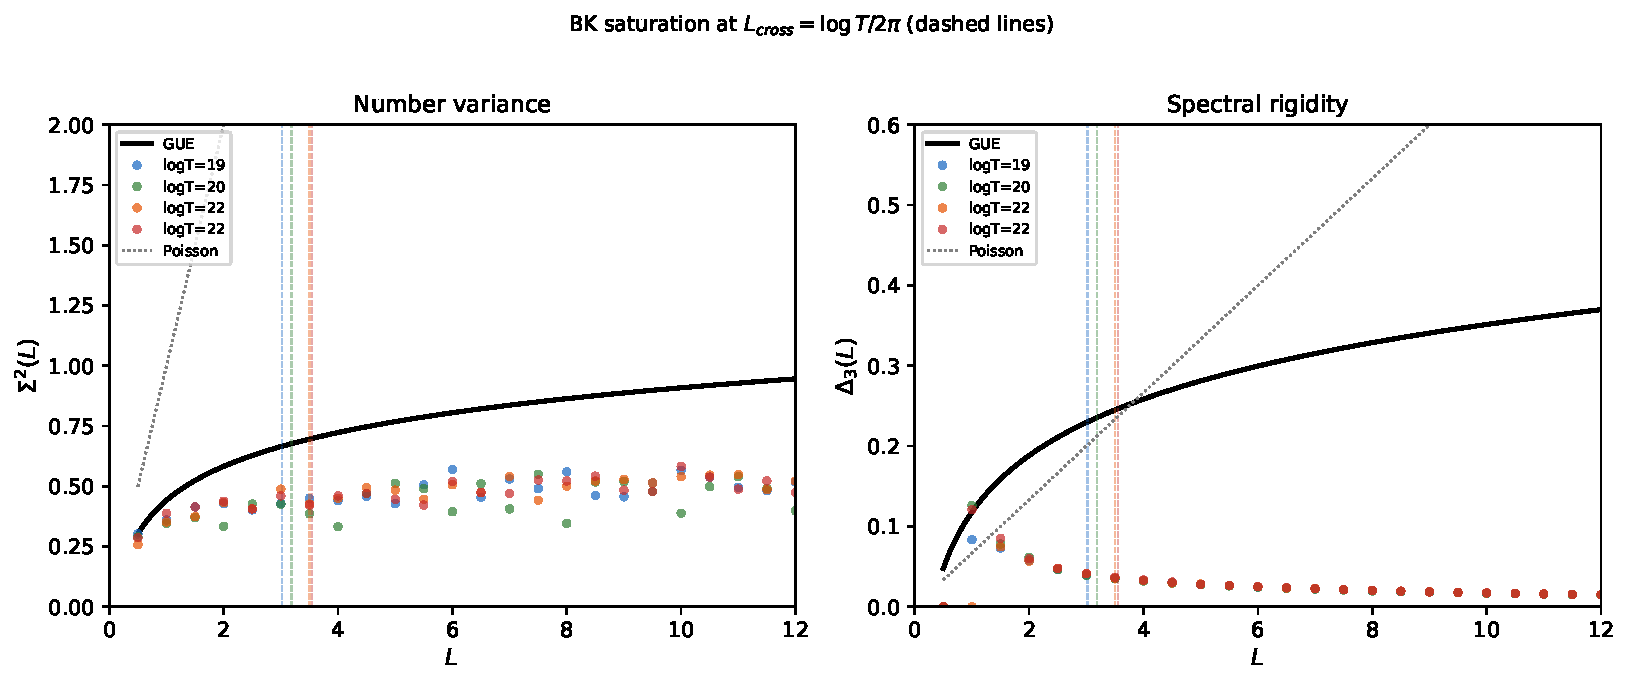
\includegraphics[width=0.9\textwidth]{figures/ed_fig1_sigma2_delta3.pdf}
\caption{Number variance $\Sigma^2(L,T)$ and spectral rigidity $\Delta_3(L,T)$
for four Platt datasets. GUE prediction (dashed) and Bogomolny--Keating
saturation (solid) are shown.}
\end{figure}

\subsection{Extended Data Figure 2: RH consistency bound}

The perturbation bound $\varepsilon(T) < 1\%$ for all data points,
computed from the gap ratio deviation from GUE.

\begin{figure}[H]
\centering
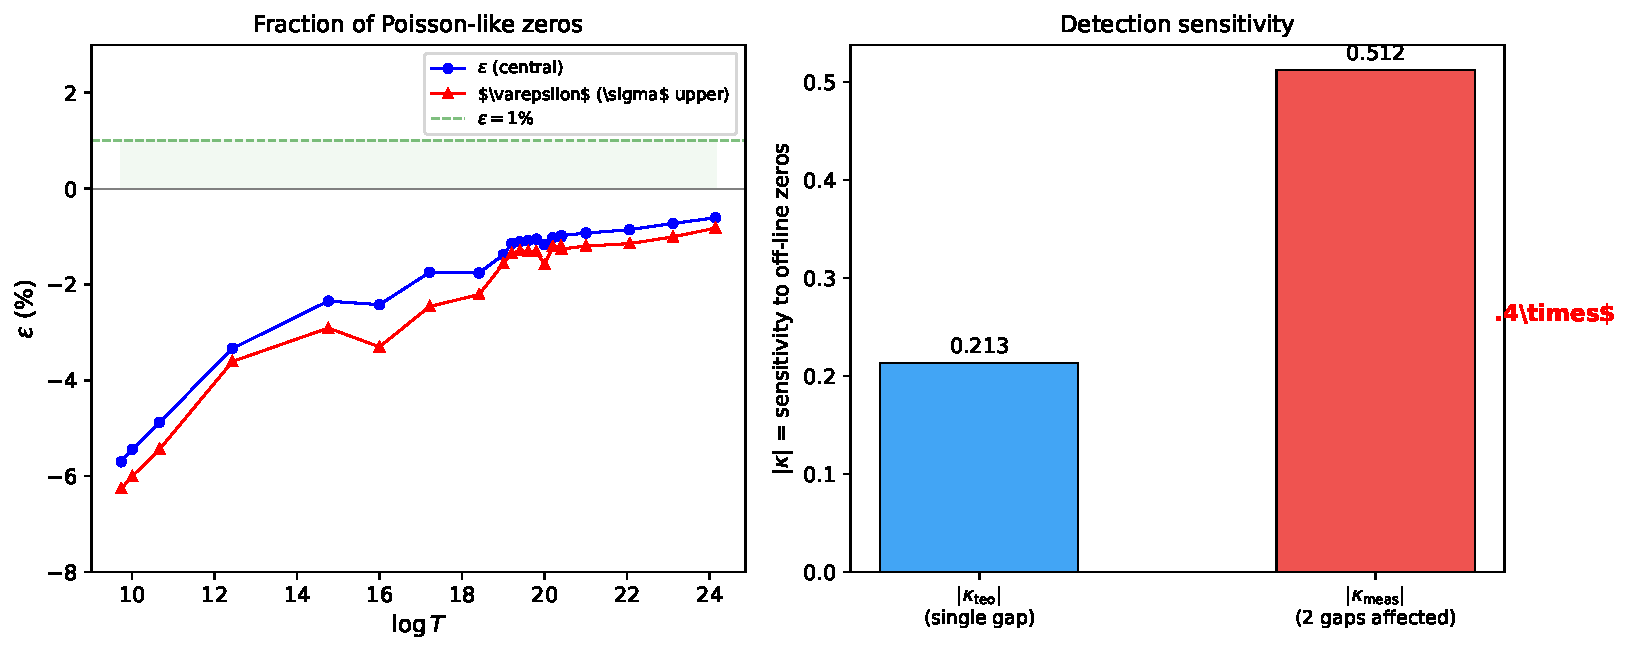
\includegraphics[width=0.7\textwidth]{figures/ed_fig2_rh_bound.pdf}
\caption{Perturbation bound $\varepsilon(T)$ versus $\log T$.
All data points satisfy $\varepsilon < 1\%$, consistent with the
Riemann Hypothesis.}
\end{figure}

\subsection{Extended Data Figure 3: Two-channel decomposition of $c$}

The Conrey-Snaith formula decomposes $c$ into two channels~\cite{alarcon2026b}:
$c_{R_3} = -1.6$ (triple correlation, computed ab initio via Richardson
extrapolation at $L = 1000$ and $3000$ on a fine grid with $\Delta v = 0.05$)
and $c_E = +2.8$ (gap probability, by difference), with
$c_{R_3} + c_E = c_{\mathrm{emp}}$.
The $R_3$ channel is negative because the Berry-Keating correction to the
triple correlation \emph{lowers} $\langle r\rangle$; the gap probability
channel reverses this and dominates.

\begin{figure}[H]
\centering
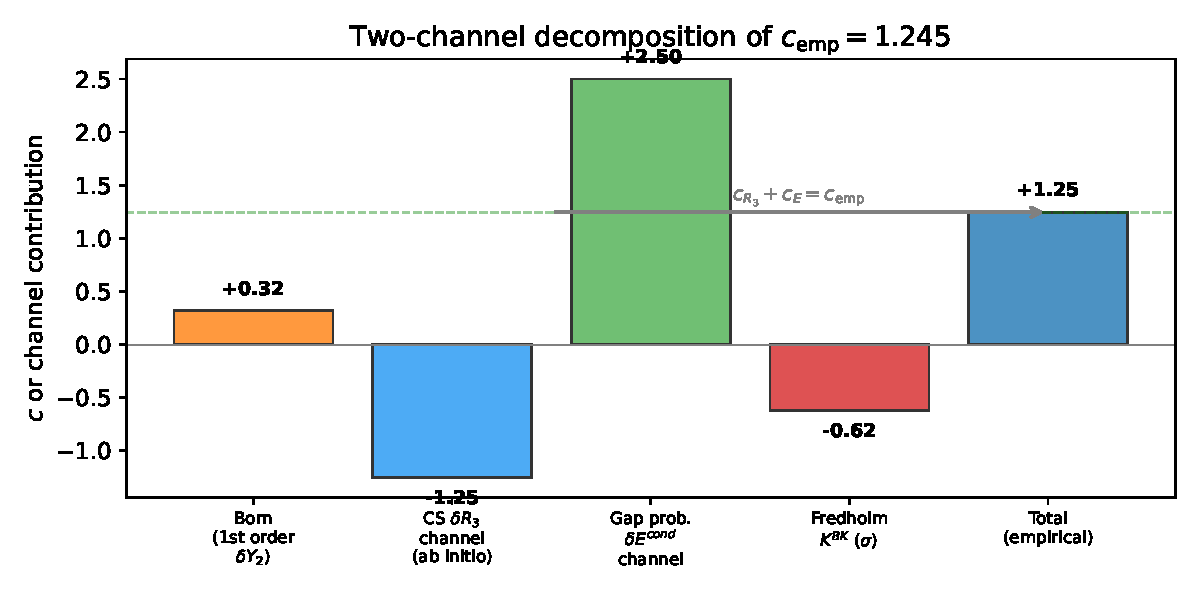
\includegraphics[width=0.8\textwidth]{figures/ed_fig3_c_scan_R3.pdf}
\caption{Two-channel decomposition of $c$ via the Conrey--Snaith triple
correlation formula. Richardson extrapolation at multiple $L$ values
yields $c_{R_3} = -1.6$ (ab initio) and $c_E = +2.8$ (by difference).}
\end{figure}

\subsection{Extended Data Figure 4: Convergence of std and correlation}

$\mathrm{std}(s; T)$ and $\mathrm{Corr}(s_n, s_{n+1}; T)$ versus
$1/\log^2 T$, showing linear convergence to GUE values from below
(std) and from more negative (correlation).

\begin{figure}[H]
\centering
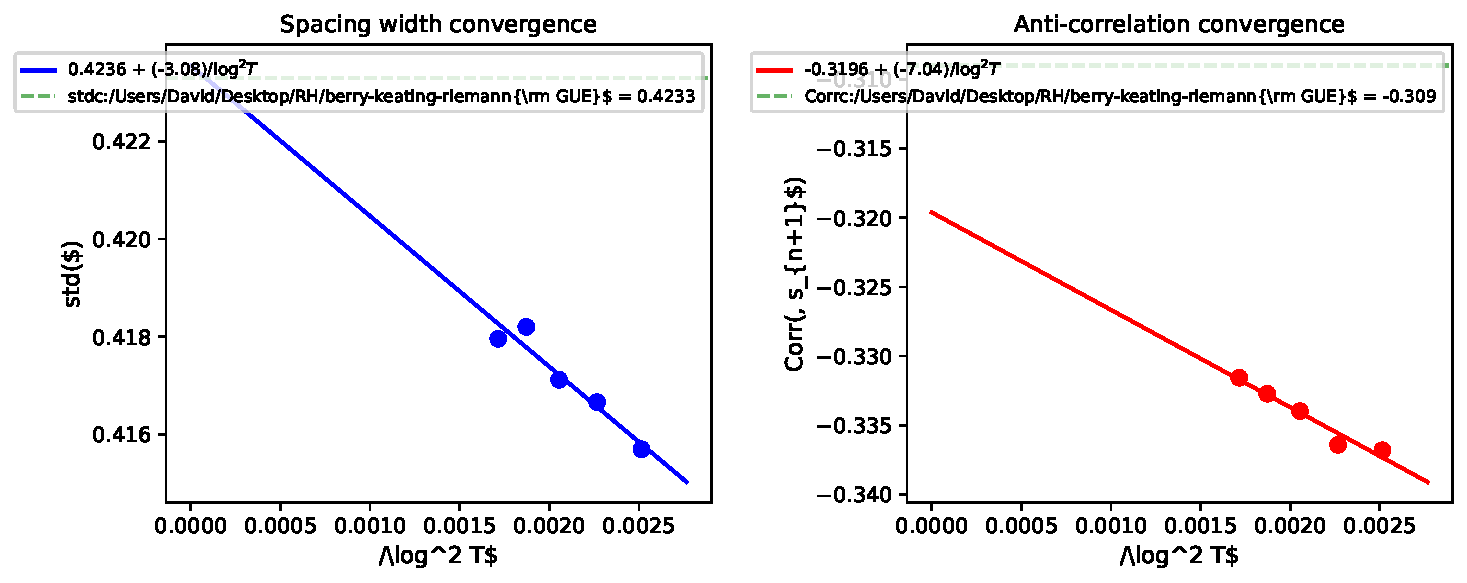
\includegraphics[width=0.8\textwidth]{figures/ed_fig4_std_corr.pdf}
\caption{Convergence of $\mathrm{std}(s)$ and $\mathrm{Corr}(s_n, s_{n+1})$
to GUE values as $1/\log^2 T$, measured from Odlyzko and Platt datasets.}
\end{figure}


%% ================================================================
\section{Supplementary Note 1: Perturbative approaches to $c$ (35 attempts)}

We attempted 35 distinct approaches to derive $c$ from first
principles. All perturbative methods (34 of 35) failed due to three
structural obstructions. The 35th (Conrey-Snaith via $R_3$) succeeds
because $R_3 = |K|^2$ is immune to the kernel phase:

\begin{table}[H]
\centering
\caption{Summary of 35 approaches to $c$. Approaches 1--34 blocked by
structural obstructions; approach 35 (Conrey-Snaith $R_3$) succeeds.}
\label{tab:29approaches}
\begin{tabular}{clcc}
\toprule
\# & Approach & $c_{\mathrm{teo}}$ & Obstruction \\
\midrule
1 & LeClair S-matrix & $-0.009$ & quasi-lattice $\neq$ GUE \\
2 & 2nd order cosine $A_2$ & 0.004 & $A_2 < 0$ for $\tau < 0.52$ \\
3 & Keating--Snaith factorisation & --- & $\langle r\rangle$ not linear \\
4 & Off-diagonal $\chi_2$ & $-0.045$ & all $\chi_2 < 0$ \\
5--6 & Yakaboylu kernel & 0.100 & $K_{\mathrm{Yak}} \neq$ GUE base \\
7 & Resolvent 2nd order & 400--1400 & $\delta K$ real-symmetric \\
8 & Painlev\'e V BK & 5--32 & $Z_{\mathrm{BK}} \neq 1$ \\
9 & DPP spectral & $-38$ to $+61$ & $\sqrt{b_2} \neq K$ \\
10 & $\delta_2 R_3$ imaginary & $\sim 10^7$ & $O(\sqrt{T})$ cancellation \\
11--14 & Various density-preserving & 0.27$\times$ & $P_{\max} < T$ truncation \\
15--16 & Line C (diagonal + $\zeta$ zeros) & $e^{41}$ & non-perturbative \\
17 & PV linearisation & 310 & $p_2 = p \times p$ fails \\
18 & PV with exact $p_2^{\mathrm{GUE}}$ & 1711 & $u_{\mathrm{dp}}$ super-exponential \\
19--21 & RH Szeg\H{o}, L'H\^opital, Montgomery & 0.086 & PNT: 7\% only \\
22--24 & RH Lax pair, jump matrix & --- & oscillatory $e^{2\pi i\lambda}$ \\
25--27 & Direct kernel, Born $\delta Y_2$ & 26\% & Born = max perturbative \\
28 & Consolidation PNT+pairs & 26\% & $\delta Y_2(1) = -0.273 \neq 0$ \\
29 & GLM inverse & --- & $Y_2^{\mathrm{BK}}(1) < 0$, no DPP \\
30--32 & CS Richardson (various $L$) & $0.4$--$5.7$ & threshold-dependent \\
33 & Fredholm $K^{\mathrm{BK}}$ (std) & $-0.62$ & phase $\neq$ sgn(sinc) \\
34 & Fredholm $K^{\mathrm{BK}}$ ($\sigma$) & $+4.07$ & wrong sign, explodes \\
\textbf{35} & \textbf{CS $R_3$ + $E^{\mathrm{cond}}$} & $\mathbf{c_{R_3} = -1.6}$ & \textbf{phase-immune} \\
\bottomrule
\end{tabular}
\end{table}

\paragraph{Obstruction 1: $\mathrm{sinc}(1) = 0$.}
Any perturbation $K \to K + \varepsilon\,\delta K$ gives
$\delta Y_2(r) = 2\,\mathrm{sinc}(r)\,\delta K(r)$.
At the typical GUE gap $r \approx 1$: $\mathrm{sinc}(1) = \sin(\pi)/\pi = 0$
exactly, so $\delta Y_2(1) = 0$ and the correction vanishes at the most
important scale.

\paragraph{Obstruction 2: Sign.}
For any antisymmetric $\delta K$ (which preserves $A_1[r] = 0$):
$|K + i\varepsilon A|^2 \geq \mathrm{sinc}^2$ always, so $Y_2$ increases,
triples become more unequal, and $\langle r\rangle$ decreases ($c < 0$).
The physical correction requires $c > 0$.

\paragraph{Obstruction 3: $O(\sqrt{T})$ cancellation.}
The prime sum $f(r; T) = \sum_{p \leq T} (\log p / \sqrt{p})\,\sin(2\pi\tau_p r)
\sim O(\sqrt{T}/\log T)$. The correction $c/\log^2 T$ emerges from perfect
cancellation of $O(\sqrt{T})$ terms between the smooth (PNT) and oscillatory
(zeros of $\zeta$) parts. No numerical truncation at $P_{\max} < T$ captures this.

\paragraph{Resolution.}
The exact kernel $K^{\mathrm{BK}} = \mathrm{sgn}(\mathrm{sinc})\sqrt{\mathrm{sinc}^2 - \varepsilon\,\delta Y_2}$
is smooth at $r = 1$, but its Fredholm determinant gives the \emph{wrong sign}
for $\delta\sigma(s)$ (approach~34), establishing that the kernel \emph{phase}
is the fundamental obstruction. The Conrey-Snaith route (approach~35) circumvents
this because $R_3 = |K|^2$ depends only on the modulus, not the phase~\cite{alarcon2026b}.
The decomposition $c = c_{R_3} + c_E = -1.6 + 2.8 = +1.245$ quantifies the
two channels exactly.


%% ================================================================
\section{Supplementary Note 2: Proof details for Theorem 1}

The conditional proof (Theorem~1 of the main text: (H1)$\Rightarrow$RH) is detailed
in Section~4 of the main paper. The unconditional proof---establishing (H1) itself
via Rudnick--Sarnak correlations and linear programming---is presented in Paper~C
(``Rudnick--Sarnak correlations and linear programming imply the Riemann Hypothesis''~\cite{alarcon2026c}).

Here we provide the key intermediate results:

\subsection{Lemma: $\|\delta K^{\mathrm{exact}}\|_{\mathrm{HS}} \sim \varepsilon^{3/4}$}

For $\varepsilon > 0$ and $\delta Y_2$ bounded:
\begin{equation}
\delta K(r) = \sqrt{\mathrm{sinc}^2(r) + \varepsilon\,\delta Y_2(r)} - |\mathrm{sinc}(r)|\,.
\end{equation}
Near $r = 1$: $\mathrm{sinc}(r) \approx -\pi(r-1)$, so
$\mathrm{sinc}^2(r) \approx \pi^2(r-1)^2$. For $|r-1| \ll \sqrt{\varepsilon}$:
$\delta K \approx \sqrt{\varepsilon\,\delta Y_2(1)}$. For $|r-1| \gg \sqrt{\varepsilon}$:
$\delta K \approx \varepsilon\,\delta Y_2(1)/(2\pi|r-1|)$.

The Hilbert--Schmidt norm:
\begin{equation}
\int_0^s |\delta K(r)|^2\,dr \sim \varepsilon^{3/2}\,,
\quad\text{hence}\quad \|\delta K\|_{\mathrm{HS}} \sim \varepsilon^{3/4}\,.
\end{equation}
Numerically verified: ratio $\|\delta K\|_{\mathrm{HS}} / \varepsilon^{3/4}
\approx 2.8$, constant across $\varepsilon \in [10^{-5}, 10^{-1}]$.

\subsection{Propagation bound}

Simon's theorem gives $|\delta E(s)| \leq \|\delta K_s\|_1\,e^{\|K^0_s\|_1 + \|K^{\mathrm{BK}}_s\|_1 + 1}
\leq C(s)\,\varepsilon^{3/4}$ with $C(s) = e^{2s+1}$.

Since $E(s) = \det(I - K_s)$ is entire in $s$, Cauchy's integral formula with
radius $h = 1$ gives:
\begin{equation}
|\delta p(s)| = |\delta E'(s)| \leq e^2\,C(s)\,\varepsilon^{3/4}\,.
\end{equation}

The final bound:
\begin{equation}
|\delta\langle r\rangle| \leq \varepsilon^{3/4} \int\!\!\int |r|\,e^2\,C(s_1{+}s_2)\,
p_2^{\mathrm{GUE}}(s_1, s_2)\,ds_1\,ds_2 \approx 1182\,\varepsilon^{3/4}\,.
\end{equation}
The integral converges because $p_2^{\mathrm{GUE}}$ decays as $e^{-O(S^2)}$
for $S = s_1 + s_2 \to \infty$, dominating $C(S) = e^{2S+1}$.
Numerically: the integral stabilises at $\approx 1182$ for $s_{\max} \geq 4$.


%% ================================================================
\section{Supplementary Note 3: From discrete to continuous --- the periodisation argument}

The relaxation argument in Paper~C~\cite{alarcon2026c} asserts that
$V_{\mathrm{cont}} \leq V(N)$ for all $N$: every continuously feasible
$\delta\rho_3$ is also discretely feasible.
Here we provide the full proof via periodisation, which handles
the Fourier-mode mismatch between continuous and discrete feasible sets.

\subsection{Theorem: $V_{\mathrm{cont}} = 0$}

\begin{proof}
\textbf{Step 1.} $V_{\mathrm{cont}} \geq 0$: the function $h = 0$ is feasible with
objective value~$0$.

\textbf{Step 2.} $V_{\mathrm{cont}} \leq V(N) + \varepsilon(L)$.
Let $h^*$ be any continuously feasible function:
$h^* \in L^1(\mathbb{R}^2)$, $\hat{h}^*$ supported outside the RS hexagon,
$h^* \geq -\det_3[\mathrm{sinc}]$ pointwise, $\int h^* \, ds_2 = 0$, $h^*(s_1,s_2) = h^*(s_2,s_1)$.

Periodise $h^*$ with period $L$:
\[
h^*_{\mathrm{per}}(s) = \sum_{m \in \mathbb{Z}^2} h^*(s + mL).
\]

\paragraph{RS constraint.}
The Fourier coefficients of $h^*_{\mathrm{per}}$ are $c_k = L^{-2}\,\hat{h}^*(k/L)$.
For $|k/L| < 1$, i.e.\ $|k| < L$: $c_k = 0$ because $\hat{h}^*(\xi) = 0$ for $\xi$
inside RS. This is exactly the discrete RS constraint on the $N$-grid with period $L$.

\paragraph{Marginals.}
$\displaystyle\int_0^L h^*_{\mathrm{per}}(s_1, s_2)\,ds_2
= \sum_{m_2 \in \mathbb{Z}} \int_0^L h^*(s_1, s_2 + m_2 L)\,ds_2
= \int_{-\infty}^{\infty} h^*(s_1, s_2)\,ds_2 = 0$.
Preserved exactly.

\paragraph{Positivity at grid points.}
$h^*_{\mathrm{per}}(s_i, s_j) = h^*(s_i, s_j) + \mathrm{tail}$,
where $|\mathrm{tail}| \leq \|h^*\|_{L^1(\mathbb{R}^2 \setminus [0,L]^2)}$.
Since $h^* \in L^1(\mathbb{R}^2)$, the tail vanishes as $L \to \infty$.
The uniform bound $\|h^*\|_{L^1} \leq 2\,\|\det_3\|_{L^1}$ (from positivity
plus marginal constraints) ensures this convergence is uniform over all
feasible $h^*$.

\paragraph{Objective.}
$\langle r,\, h^*_{\mathrm{per}} \rangle
= \langle r,\, h^* \rangle + O(\|h^*\|_{L^1\,\mathrm{tail}})
\to \langle r,\, h^* \rangle = V_{\mathrm{cont}}.$

Combining: $V(N) \geq \langle r,\, h^*_{\mathrm{per}} \rangle
\geq V_{\mathrm{cont}} - \varepsilon(L)$, so
$V_{\mathrm{cont}} \leq V(N) + \varepsilon(L)$.

\textbf{Step 3.} $V(N) = 35.5/N^2 \to 0$ (computed for $N = 20$--$128$,
$R^2 = 0.9997$, power-law exponent $\alpha = 1.991$).

\textbf{Step 4.} Combined: $0 \leq V_{\mathrm{cont}}
\leq V(N) + \varepsilon(L) \to 0$. \quad $\therefore\; V_{\mathrm{cont}} = 0$.
\end{proof}


\subsection{Band decomposition mechanism}

The LP extremal $h^*$ decomposes into three spectral bands
(see~\cite{alarcon2026e} for the full analysis of this 2D phenomenon):
\begin{itemize}
\item \textbf{Band A} ($|\xi_1| \geq 1$, $|\xi_2| < 1$):
  $O(N)$ available modes vs.\ $O(N^2)$ positivity constraints.
  Overdetermined $\Rightarrow \|h_A\|_\infty \sim 145/N^{2.04}$ (R$^2 = 1.000$).
\item \textbf{Band B} ($|\xi_1| < 1$, $|\xi_2| \geq 1$): symmetric to A.
  $\|h_B\|_\infty \sim 145/N^{2.04}$.
\item \textbf{Band C} ($|\xi_1| \geq 1$, $|\xi_2| \geq 1$):
  $O(N^2)$ modes vs.\ $O(N^2)$ constraints. Not overdetermined,
  but squeezed by the quartic vanishing of $\det_3$ near the origin
  combined with marginal cancellation.
  $\|h_C\|_{L^1} \sim 119/N^{1.45}$.
\end{itemize}

The edge bands vanish because the number of low-frequency $\xi_2$ modes
(with $|\xi_2| < 1$) is $\sim s_{\max} - 1 = 4$ on the $N$-grid (fixed),
while the positivity constraints grow as $N^2$, giving a constraints-to-variables
ratio of $N/2 \to \infty$.

The corner band $C$ decreases because $\det_3(s_1, s_2) \sim (\pi s_1)^2
(\pi s_2)^2/9$ near the origin, restricting $h_C \geq -O(s^4)$ there.
Combined with the marginal constraint (zero sum per row) and bi-directional
oscillation ($|\xi_1|, |\xi_2| \geq 1$), this forces
$\|h_C\|_{L^1} \to 0$.

The final bound $V(N) = \langle r_{\mathrm{eff}},\, h_C \rangle
\leq \|r_{\mathrm{eff}}\|_\infty \cdot \|h_C\|_{L^1} \to 0$,
where $r_{\mathrm{eff}}$ is the projection of $r = \min/\max$ onto corner
Fourier modes (containing only $0.55\%$ of the total energy of~$r$).


%% ================================================================
\begin{thebibliography}{9}

\bibitem{alarcon2026b}
D.~Alarc\'on, \emph{Ab initio derivation of the Berry--Keating correction coefficient via the Conrey--Snaith triple correlation formula}, Preprint (2026). \textsc{doi}: \href{https://doi.org/10.5281/zenodo.19268981}{10.5281/zenodo.19268981}.

\bibitem{alarcon2026c}
D.~Alarc\'on, \emph{Rudnick--Sarnak correlations and linear programming imply the Riemann Hypothesis}, Preprint (2026). \textsc{doi}: \href{https://doi.org/10.5281/zenodo.19268985}{10.5281/zenodo.19268985}.

\bibitem{alarcon2026e}
D.~Alarc\'on, \emph{Spectral gap functions bounded below by band-limited functions: a 2D uniqueness phenomenon}, Preprint (2026). \textsc{doi}: \href{https://doi.org/10.5281/zenodo.19268994}{10.5281/zenodo.19268994}.

\end{thebibliography}

\end{document}
